\chapter{Iteracion 6: Implementacion de un sistema gestionador para la placa de instrumentacion} % (fold)
\label{cha:iteracion_6}

\section{Introduccion} % (fold)
\label{sec:introduccion}

El sistema de instrumentacion recibe, interpreta y distribuye datos de sensores, para luego enviarselas a otro sistema que extiende las funciones del primero, teniendo entonces un sistema de gestion y administracion para los datos de los sensores. En esta iteracion, realizamos una implementacion de este ultimo sistema. La idea es tener un sistema cuyas funciones incluyan el manejo de la placa de instrumentacion, pero que ademas, permita un uso mas general en lo que respecta al manejo de sistemas administradores de sensores y actuadores
La figura \ref{fig:topologiaplacas} muestra una topologia basica que describe el rol de este sistema a implementar.

% section introduccion (end)

\section{Requerimientos de la iteracion} % (fold)
\label{sec:requerimientos_de_la_iteracion}

\begin{itemize}
\item El sistema deberia estar implementado en una placa de desarrollo de manera que se pueda conectar a la placa de instrumentacion via comunicacion serial
\item Deberia estar en el mismo lugar fisico que la placa de alimentacion.
\item Deberia implementar un servidor web con una interfaz grafica de usuario. Esta interfaz deberia permitir:
\begin{itemize}
	\item Las mismas acciones que si el usuario se conectara directamente con la placa de instrumentacion via interfaz de comando, solamente que via interfaz grafica.
	\item Enviar cualquier comando que pueda ser interpretado por la placa de instrumentacion
	\item Establecer intervalos de tiempo usando hora y fecha en los que se debe medir sobre cierto canal
\end{itemize}
\item Deberia guardar datos de mediciones e informacion sobre transacciones en general entre ambas placas en una base de datos local, accesible via la interfaz grafica 
\item La conexion entre el sistema y el usuario (dispositivo del usuario) deberia ser via Wi-Fi o algun otro protocolo inalambrico
\end{itemize}


% section requerimientos_de_la_iteracion (end)

\section{Desarrollo} % (fold)
\label{sec:desarrollo}

\subsection{Placa de desarrollo elegida para la implementacion} % (fold)
\label{sub:placa_de_desarrollo_elegida_para_la_implementacion}

Sin una seleccion previa teniendo en cuenta los requisitos, y por una cuestion de accesibilidad, se decidio implementar este sistema en una placa de desarrollo Raspberry Pi B+ (figura \ref{fig:raspberrypi}), embebida con un sistema operativo Raspbian (Debian para Raspberry). Bajo estas condiciones, es posible cubrir todos los requerimientos.

\begin{figure}[h]
  \centering
  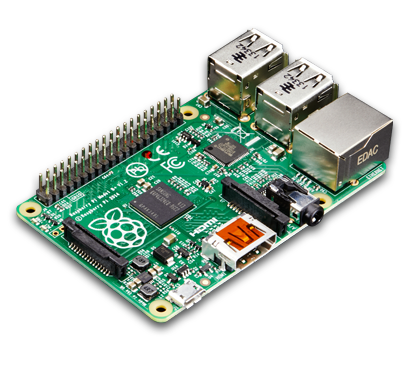
\includegraphics[width=0.80\textwidth, height = 7cm]{raspberrypi}
  \caption{Placa de desarrollo Raspberry Pi B+}\label{fig:raspberrypi}
\end{figure}
% subsection placa_de_desarrollo_elegida_para_la_implementacion (end)

\subsection{Servidor web} % (fold)
\label{sub:servidor_web}

% subsection servidor_web (end)

\subsection{Base de datos} % (fold)
\label{sub:base_de_datos}

% subsection base_de_datos (end)

\subsection{Interfaz grafica de usuario} % (fold)
\label{sub:interfaz_grafica_de_usuario}

% subsection interfaz_grafica_de_usuario (end)

% section desarrollo (end)

\section{Pruebas} % (fold)
\label{sec:pruebas}

% section pruebas (end)

\section{Resultados} % (fold)
\label{sec:resultados}

% section resultados (end)

% chapter iteracion_6 (end)